%!TeX spellcheck = en-US
%!TEX root = ../hw1_report.tex
\subsection{$(a,b)$}

We identify three eigenvalues $\lambda_{1}$, $\lambda_{2}$ and $\lambda_{3}$ as outliers in $\mathbb{C}$. A crude estimate for the rate of convergence for eigenvalue $\lambda_{i}$ is given by
\begin{equation*}
  \varepsilon_{i}^{(m)}\leq \frac{\rho^{m-1}}{|\lambda_{i} - c|^{m-1}}.
\end{equation*}
Thus the circles with centre $c_{i}$ and radius $\rho_{i}$ give the convergence estimate. They are plotted in \ref{fig_task6a} together with the eigenvalues, where the outliers are marked. The corresponding values are
\begin{align*}
&\lambda_{1} \approx -47.016 + i 0.166,\,&c_{1} = -5+i0.5,\,&\rho_{1} = 14,\,&\varepsilon_{1}^{m}\leq (0.33)^{m-1}\\ &\lambda_{2} = 1.314 + i 12.664,\,&c_{2} = -23-i6,\,&\rho_{2} = 25,\,&\varepsilon_{2}^{m}\leq (0.82)^{m-1} \\ &\lambda_{3} = 0.986 - i11.898,\,&c_{3} = -23+i9,\,&\rho_{3} = 26,\,&\varepsilon_{2}^{m}\leq (0.82)^{m-1}
\end{align*}


\begin{figure}[h!]
\centering
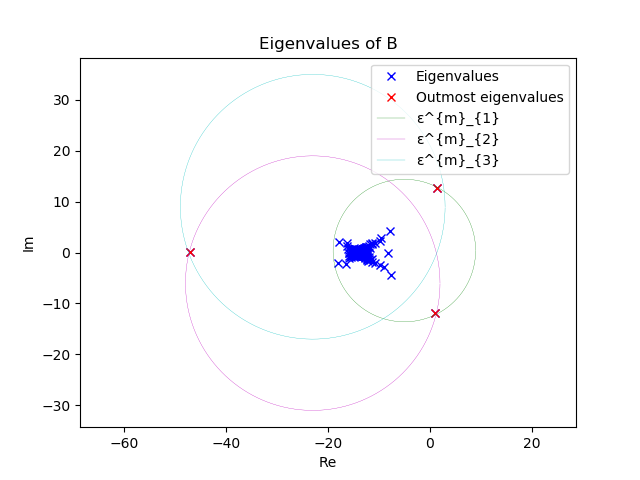
\includegraphics[scale=0.8]{../task6/task6a.png}
\caption{The eigenvalues of $B$, with the outliers marked and the corresponding circles.}
\label{fig:task6a}
\end{figure}

\subsection{$(c)$}
We expect the fastest convergence for $\lambda_{1}$, motivated by $\varepsilon_{1}^{m}\leq (0.33)^{m-1}$. The eigenvalue error for $\lambda_{1}$ for Arnoldi method, with double GS for $m = 2, 4, 8, 10, 20, 30, 40$ is plotted in \ref{fig:task6c1}. About $m = 14$ gives an eigenvalue error less than $10^{-10}$.

In \ref{fig:task6c2} we have plotted the evolution of the Ritz values as $m$ increases. As predicted are $\lambda_{1}$, $\lambda_2$ and $\lambda_{3}$ the first to converge.
\begin{figure}[h!]
\centering
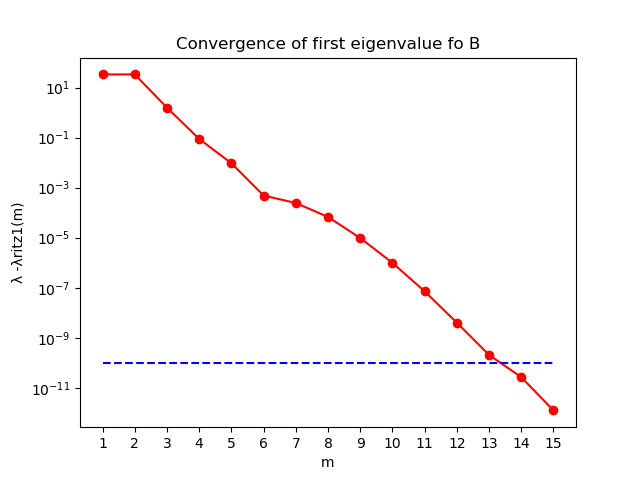
\includegraphics[scale=0.8]{../task6/task6c_eigConv.png}
\caption{Comparison of eigenvalues after $m$ iterations.}
\label{fig:task6c1}
\end{figure}

\begin{figure}[h!]
\centering
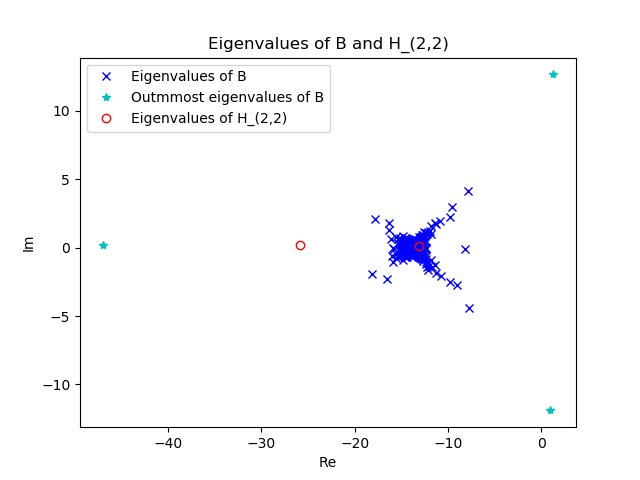
\includegraphics[scale=0.4]{../task6/task6c_m2.png}
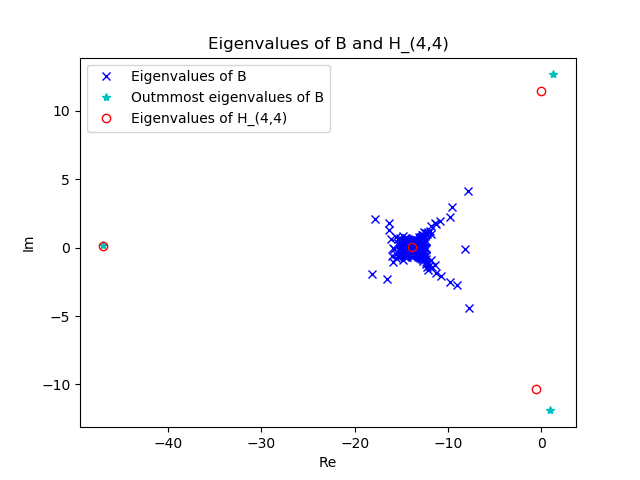
\includegraphics[scale=0.4]{../task6/task6c_m4.png}
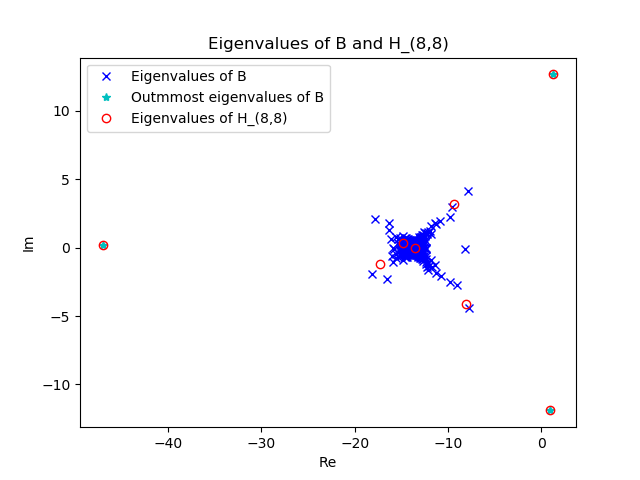
\includegraphics[scale=0.4]{../task6/task6c_m8.png}
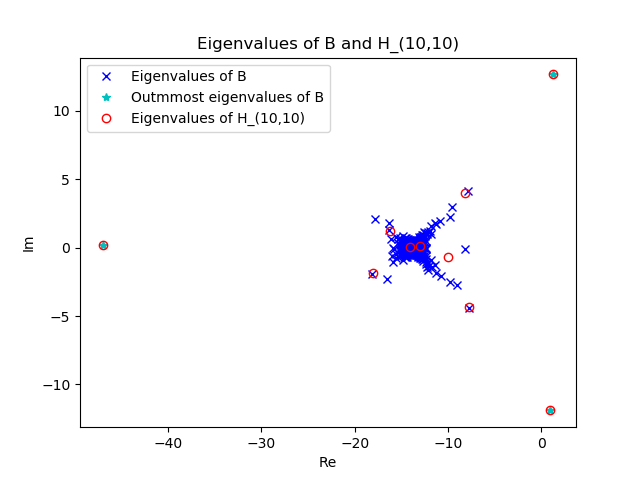
\includegraphics[scale=0.4]{../task6/task6c_m10.png}
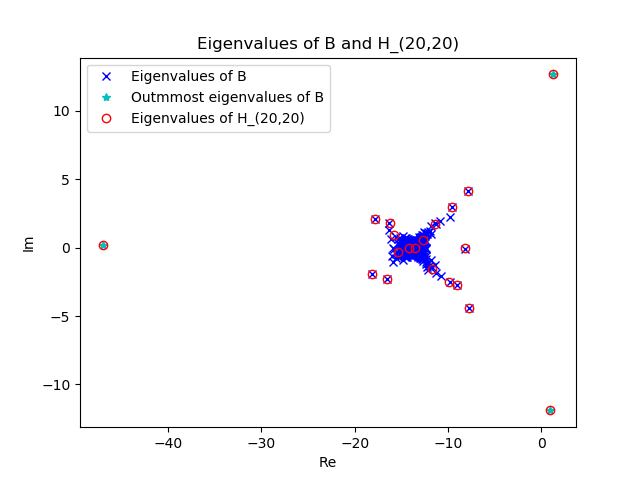
\includegraphics[scale=0.4]{../task6/task6c_m20.png}
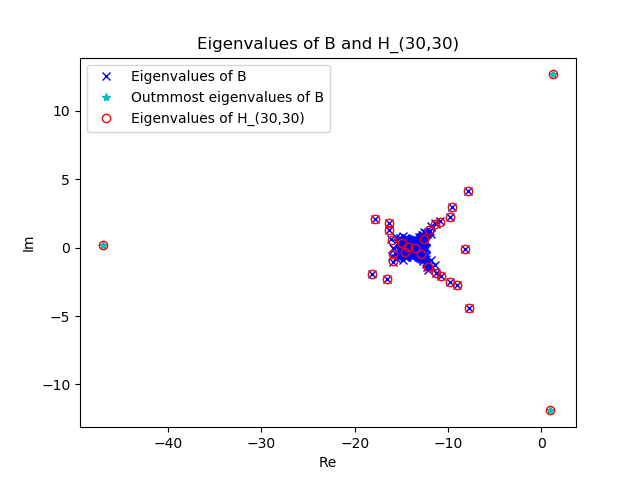
\includegraphics[scale=0.4]{../task6/task6c_m30.png}
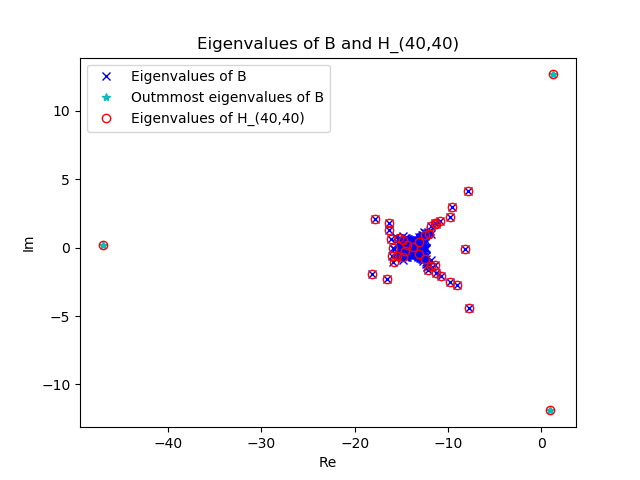
\includegraphics[scale=0.4]{../task6/task6c_m40.png}

\caption{The eigenvalues of $B$, with the outliers marked, and the Ritz values for the Arnoldi method, with double GS for $m = 2, 4, 8, 10, 20, 30, 40$.}
\label{fig:task6c2}
\end{figure}

\subsection{$(d)$}
\begin{figure}[h!]
\centering
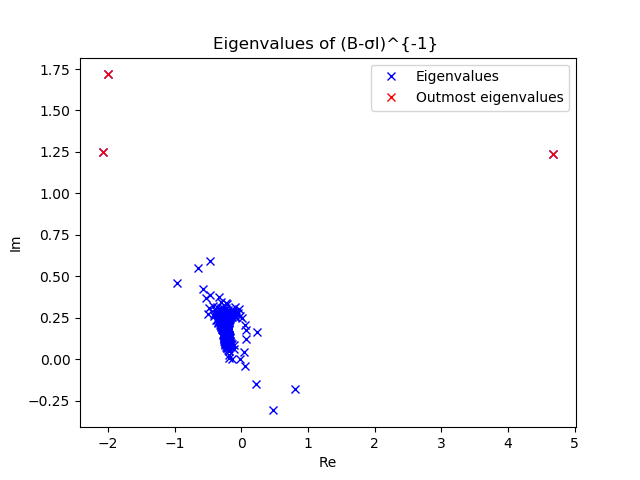
\includegraphics[scale=0.8]{../task6/task6d.png}
\caption{The eigenvalues of $(B-\sigma I )^{-1}$, with the outliers marked.}
\label{fig:task6d}
\end{figure}
\subsection{$(e)$}
From Figure \ref{fig:task6e1} we read that about $12$ iterations are required for an eigenvalue error about $10^{-10}$, i.e. Arnoldi's method with shift-invert is faster than standard Arnoldi's method. This increase in convergence should not be exaggerated, as theory says that they should be about the same. The idea of shift and invert is to transform the spectrum such that eigenvalues close to $\sigma$ becomes an outlier. But with $\sigma = -11 + i2$ we read from \ref{fig:task6d} that the outliers are the same as for $B$, i.e. the transformed spectrum has not changed considerably.
\begin{figure}[h!]
\centering
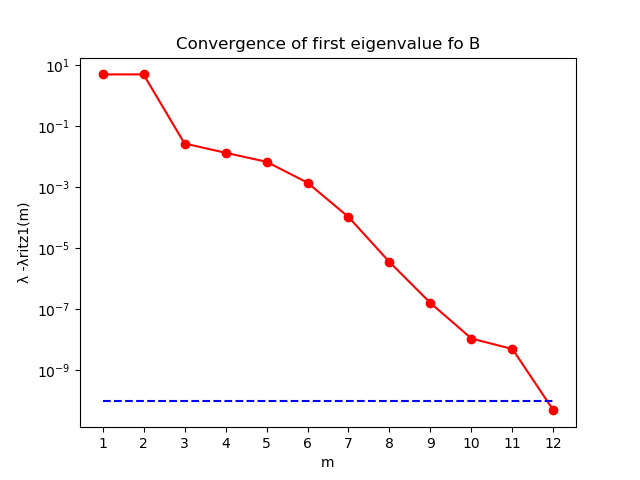
\includegraphics[scale=0.8]{../task6/task6e_eigConv.png}
\caption{Comparison of eigenvalues after $m$ iterations with shift and invert.}
\label{fig:task6e1}
\end{figure}
